\begin{frame}
    \frametitle{Problems}

    \begin{itemize}
        \item Aseptic loosening \begin{itemize}
            \item Reduction in bone strain and a non-physiological distribution of load
        \end{itemize}
        \item Relevant only for amputees
    \end{itemize}

\end{frame}

\begin{frame}
    \frametitle{Alternatives}

    \begin{itemize}
        \item Brånemark \footcite{KANG20101130}: \begin{itemize}
            \item Inappropriate cutanous integration
            \item Two surgical steps
            \item Prone to bending, fractures and loosening
        \end{itemize}
        \begin{figure}[h]
        \centering
            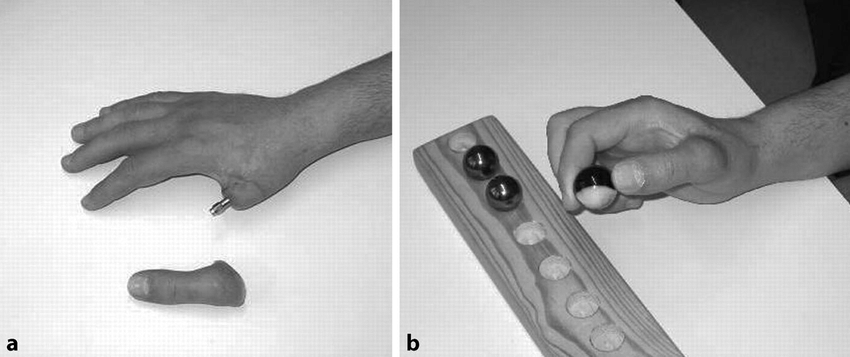
\includegraphics[width=0.6\textwidth]{figures/branemark-thumb.png}
        \caption{{ Brånemark thumb prosthesis \footcite{Li2017Branemark} }}
        \end{figure}
    \end{itemize}

\end{frame}